\documentclass{imcs}
\usepackage[T2A]{fontenc}
\usepackage[utf8x]{inputenc}
\usepackage[russian]{babel}
\usepackage{graphicx}
\usepackage{hyperref}
\usepackage{enumitem}
\usepackage{listings}

\title{Реализация замыканий для языка программирования Pascal}
\author{Кевролетин Василий Владимирович}
\mentorinfo{старший преподаватель}
\mentorname{А.С.~Кленин}
\year{2013}



\begin{document}
\maketitle

\tableofcontents
\pagebreak

\section*{Аннотация}
\addcontentsline{toc}{section}{Аннотация}
Цель данной работы - реализовать поддержку замыканий в компиляторе Free Pascal Compiler.
Рассмотрены подходы к решению проблемы и осуществлена пробная реализация.

\pagebreak

\section{Введение}
\subsection{Глоссарий}

Анонимная функция -- функция, не имеющая идентификатора; доступна для
вызова либо в момент создания, либо, позднее, через ссылку на функцию,
хранящуюся в переменной.

Анонимный метод -- реализация замыканий в языке программирования Delphi. 

Генератор кода -- часть компилятора, обеспечивающая создание
ассемблерного кода исходной программы по ее синтаксическому дереву.

Замыкание -- функция или ссылка на функцию вместе с используемым ею
окружением; замыкание сохраняет окружение и позволяет функции
обращаться к нему даже если она вызвана за пределами лексического
пространства где была создана.

Захваченная переменная -- переменная, используемая в теле замыкания,
объявленная во внешнем для замыкания лексическом пространстве.

Парсер -- часть компилятора, обеспечивающая создание синтаксического
дерева.

Свободная переменная -- переменная, используемая в теле функции, но не
являющейся параметром или локальной переменной этой функции. Так же встречается название
``нелокальная переменная''.

Синтаксическое дерево -- иерархическая упорядоченная структура,
состоящая из узлов, хранящих информацию об объектах, используемых в
программе.

Управляемый тип данных -- для работы с динамической памятью управляемых объектов
компилятор использует специальные техники, такие как подсчёт ссылок\cite{delhpimanged}.

Функциональное программирование -- парадигма программирования,
рассматривающая вычисление как применение математических функций,
отрицающая понятие состояния и изменяемых данных. Делает акцент на
применении функций, а не на изменении состояния.

\subsection{Описание предметной области}

\paragraph{Free Pascal Compiler (FPC)} FPC -- компилятор языка Pascal с открытым исходным
кодом, поддерживающий несколько диалектов Pascal и генерирующий код для большого
числа процессорных архитектур и операционных систем \cite{fpc}. Это открытый проект,
разрабатываемый постоянной командой добровольцев и периодически получающий доработки от
сторонних разработчиков.

Как правило, компилятор выполняет только часть работы по созданию исполняемого файла.
Широко распространённой является схема \cite{dragonbook}:
\begin{enumerate}
    \item Препроцессор.
    \item Компилятор.
    \item Ассемблер.
    \item Компоновщик.
\end{enumerate}

FPC объединяет в себе препроцессор, компилятор, и, для некоторых платформ,
компоновщик. Кроме того парсер FPC используется интегрированной средой разработки
Lazarus \cite{lazarus}.

Процесс компиляции представляет собой последовательность фаз, каждая из которых
преобразует одно из представлений исходной программы в другое. Типичное разложение
компилятора на фазы \cite{dragonbook}:
\begin{enumerate}
    \item Лексический анализ.
    \item Синтаксический анализ.
    \item Семантический анализ.
    \item Генерация промежуточного кода.
    \item Машинно-независимая оптимизация.
    \item Генерация кода.
    \item Машинно-зависимая оптимизация.
\end{enumerate}

Выдающаяся особенность FPC - поддержка нескольких диалектов Pascal 
и большого числа целевых процессорных архитектур. Исходный код FPC написан со
стремлением минимизировать количество повторяющегося программного кода,
работающего в случае разных комбинаций
диалекта языка и результирующей платформы. Поэтому для каждой целевой платформы
в компиляторе FPC реализован отдельный генератор кода (все остальные части остаются
неизменными). В режимах совместимости с различными диалектами Pascal лексический,
синтаксический и семантический анализаторы работают немного по-разному. Благодаря этому
компилятор может иметь различную реализацию одной концепции языка в разных режимах
совместимости.

FPC находится в состоянии активной разработки. Разработчики постоянно улучшают компилятор,
добавляя новые возможности, оптимизации, поддержку новых платформ и исправляя ошибки\cite{fpc}. Одной из новых возможностей, которую разработчики и пользователи FPC хотят увидеть в
своём компиляторе, является поддержка замыканий.

\paragraph{Замыкания} В современных языках программирования замыкание это практическая реализация
идеи лябмда-исчесления о том, что функция может использовать в своём теле свободные
переменные (не являющиеся параметрами этой функции). В лямбда-исчислении
переменные неизменяемые, поэтому для вычисления значения функции, использующей
свободные переменные, достаточно подставить значения свободных переменных в тело
функции.

В современных императивных языках программирования переменные изменяемые.
Поэтому результат выполнения функции зависит не только от значений параметров
функции, но и от значения свободных переменных, используемых в её теле. В качестве
свободных переменных могут выступать глобальные переменные и локальные переменные
других функций. Глобальные переменные доступны в течении всего времени выполнения программы.
Однако срок жизни
локальных переменных ограничен временем работы функции, в которой они объявлены.
Особенность замыканий состоит в том, они не только могут получать доступ к любым
доступным в текущем лексическом пространстве переменным, но, к тому же, могут
обращаться к ним, даже если будут вызваны в другом лексическом пространстве, где
использованные переменные уже недоступны.

Если замыкание ссылается на локальную переменную объемлющей функции, то такая переменная 
называется «захваченной»(англ. Captured)\cite{anonymmethods}\cite{cpp}. Существует 2
способа захвата переменных: по значению и по ссылке. В случае захвата по значения
замыкание в момент своего создания запоминает значение захваченных переменных.
Захват по значению - аналог подстановки значений свободных переменных в лямбда-исчислении.
В случае захвата по ссылке, в момент своего создания замыкание запоминает ссылку 
на захваченную переменную. Сложность реализации захвата переменных по ссылке состоит в том,
что на одну переменную могут одновременно ссылаться несколько замыканий и несколько
выполняющихся функций.

\paragraph{Описание совместной деятельности}

Компилятор распространяется под лицензией GNU GPL. Разрабатывается
постоянной командой добровольцев и принимает доработки от сторонних разработчиков.
Исходный код написан на языке Freepascal. Разработка ведётся с использованием системы
контроля версий SVN, системы контроля изменений Mantis. Команда общается при
помощи списков рассылки электронных писем.

\subsection{Неформальная постановка задачи}

Добавить в компилятор Freepascal поддержку замыканий. В режиме совместимости с 
Delhpi реализация должна вести себя так же, как и анонимные методы
Delhpi. Дополнительно рассмотреть возможность создания альтернативной улучшенной
реализации, не ограниченной требованием совместимости с Delphi.

При этом компилятор должен:
\begin{enumerate}
    \item Сохранить обратную совместимость, проходить существующие тесты. 
    \item В режиме совместимости с Delphi корректно компилировать программы,
содержащие замыкания, которые компилирует Delphi.
    \item В остальных режимах предоставить пользователям использовать замыкания,
возможно с расширенными набором возможностей и альтернативным синтаксисом.
\end{enumerate}

\paragraph{Анонимные функции}
Компилятор должен поддерживать объявление анонимных функций в теле других подпрограмм:
\begin{lstlisting}
function Factory: TProc;
begin
  Result := procedure
            begin
              Writeln;
            end;
end;
\end{lstlisting}

\paragraph{Вложенные функции}
Вложенные именованные функции должны быть реализованы в виде замыканий. Ниже пример
вложенной функции FPC.
\begin{lstlisting}    
procedure outer;
var i: Integer;

  procedure inner; begin
    i := 10;
  end;

begin
  ...
end;    
\end{lstlisting}

\paragraph{Продление жизни локальных переменных}
Без возможности захвата окружения переменная data стала бы недоступной после завершения
работы функции Factory. Каждое из созданных ниже замыканий продлевает жизнь переменной
data, и может обращаться к нему даже после окончания работы Factory. В момент второго
вызова процедуры Factory переменная data, созданная во время предыдущего вызова уже
недоступна. Поэтому каждое из созданных замыканий хранит ссылку на свой собственный
экземпляр захваченной переменной. Вызов f1() напечатает значение 10, а вызов f2()
напечатает 20.
\begin{lstlisting}
function Factory(data: Integer): TProc;
begin
  Result := procedure
            begin
              Writeln( data );
            end;
  end;
    
var f1: TProc;
begin
  f1 := Factory(10);
  f2 := Factory(20);
  f1();               { 10 }
  f2();               { 20 }
end.
\end{lstlisting}    

\paragraph{Захват по ссылке}
В языке программирования Delphi замыкания захватывают переменные по ссылке. Поэтому
возможна ситуация, когда захваченную замыканием переменную меняют из другого замыкания,
или из обычной подпрограммы. Приведённый ниже код должен напечатать значение 10.
\begin{lstlisting}
var i: Integer;
    f: TProc;
begin
  i := 0;
  f := procedure
       begin
         Writeln(i);
       end;
  i := 10;
  f();                { 10 }
end.
\end{lstlisting}

\paragraph{Захват по значению}
Рассмотреть возможность реализации захвата по значению. В примере ниже переменная
i захватывается по значению. Программа должна вывести значение 0.
\begin{lstlisting}
var i: Integer;
    f: TProc;
begin
  i := 0;
  f := procedure
       closure(i)
       begin
         Writeln(i);
       end;
  i := 10;
  f();                { 0 }
end.
\end{lstlisting}

\iffalse TODO: в качестве исключения описать здесь дискуссию из мейлинг листа
по этому поводу \fi

\paragraph{Захват по значению}
Рассмотреть возможность реализации упрощенного синтаксиса для более короткого объявления
анонимных функций. В примере ниже в метод map передаётся анонимная функция, принимающая
один аргумент типа Integer и возвращающая свой аргумент, увеличенный на 1.
\begin{lstlisting}
type TListVisitor = procedure(x: Integer);
var  list: TList;
begin
   ...
   list.map(TListVisitor is x := x + 1)
   ...
end.
\end{lstlisting}

\subsubsection{Обзор существующих методов решения}

\paragraph{Аналогичные (конкурирующие) решения}

\iffalse TODO: добавить JAVA, Scala \fi
\iffalse TODO: посмотреть с какой версии поддерживается та или иная фича, показать что замыкания совсем недавно появились во многих языках \fi

~~~

\begin{table}[h!]
\begin{center}
\begin{tabular}{|l|c|c|c|c|c|}
\hline
  ЯП     &  Анонимные  &  Вложенные  &  Захват по  &  Захват по  &  Замыкания  \\
         &  функции    &  функции    &  значению   &  ссылке     &             \\
\hline
 Perl    &  +          &  +/-        &             &  +          &  +          \\
\hline
 Python  &  +          &  +          &             &  +          &  +          \\
\hline
 Ruby    &  +          &  +          &             &  +          &  +          \\
\hline
 Scheme  &  +          &  +          &             &  +          &  +          \\
\hline
 Elisp   &  +          &  +          &             &  +          &             \\
\hline
 Scala   &  +          &  +          &             &  +          &  +          \\
\iffalse \hline
 Java    &  ?          &  ?          &  ?          &  ?          &  ?          \\ \fi
\hline
 C       &             &             &             &             &             \\
\hline
 C++     &  +          &             &  +          &  +          &             \\
\hline
 Delphi  &  +          &  +          &             &  +          &  +          \\
\hline
 Fpc     &             &  +          &             &             &             \\
\hline
\end{tabular}
\caption{Поддержка замыканий и анонимных функций современными ЯП}\label{tab:wsi_diff_rel}
\end{center}
\end{table}

\paragraph{Описание предшествующих работ}
Студенты нашей кафедры успешно развивали компилятор Fpc в рамках своих
курсовых и дипломных работ:
\begin{enumerate}
    \item Дипломная работа «Расширение компилятора Free Pascal для поддержки
обобщённого программирования». Автор Нелепа А.А. Руководитель Кленин А. С.
2007г.
    \item Курсовая работа «Анализ потоков управления для языка программирования Pascal» Автор Баль Н. В. Руководитель Кленин А. С. 2008г.
    \item Курсовая работа «Доработка компилятора Free Pascal: case of string» Автор Денисенко М. В. Руководитель Кленин А. С. 2009г.
    \item Курсовая работа «Оператор for-in для компилятора Free Pascal» Автор Лукащук М.
А. Руководитель Кленин А. С. 2010г.
\end{enumerate}

\paragraph{Вывод}
Ценность замыканий подтверждена их популярностью и востребованностью. 
Сегодня замыкания поддерживают большинство языков программирования, а программисты 
активно используют их на практике. Поэтому для поддержания компилятора FPC в 
актуальном состоянии необходимо реализовать в нём поддержку замыканий.

\subsection{План работ}

\begin{enumerate}
    \item Согласовать работу с разработчиками FPC.
    \item Изучить архитектуру и исходных код компилятора.
    \item Изучить реализацию замыканий в похожих языках программирования.
    \item Спроектировать реализацияю.
    \item Осуществить пробную реализацию.
    \item Используя полученный опыт создать окончательную реализацияю.
\end{enumerate}

\section{Требования к окружению}

FPC может компилировать свой собственный исходный код. Поэтому
список целевых платформ совпадает со списком платформ, на которых работает
FPC.

\subsection{Требования к аппаратному обеспечению}

Для работы требуется компьютер, пригодный для набора исходного кода программы.
Т.е. кроме работающих процессора, оперативной и постоянной памяти требуются
клавиатура и монитор.

Поддерживаемые архитектуры процессоров\cite{fpctargets}:
\begin{itemize}
    \item I386
    \item PowerPC
    \item Sparc
    \item AMD64 (x86-64)
    \item PowerPC64
    \item ARM
    \item m68k 
\end{itemize}

\subsection{Требования к программному обеспечению}

\paragraph{Компилятор} FPC версии 2.6 и выше
\paragraph{Операционная система}
На сайте FPC указано 53 разных поддерживаемых комбинаций архитектуры 
процессора и операционной системы\cite{fpctargets}. Здесь приведём
только популярные операционные системы, поддерживаемые компилятором
для архитектуры процессора I386:
\begin{itemize}
    \item Win32 for i386
    \item Linux for i386
    \item Target Darwin (Mac OS X) for i386 (2.1.x and later)
    \item FreeBSD/ELF for i386
    \item Android for i386
\end{itemize}
    
\subsection{Требования к пользователям}
Программисты, владеющие языком программирования Free Pascal или Delphi.

\section{Архитектура системы}

С точки зрения пользователя проект компилятора FPC состоит из нескольких 
частей:
\begin{description}
    \item[Сompiler] - программа с интерфейсом командной строки. На вход
принимает список текстовых или объектных файлов. Результат работы --
файлы с ассемблерным кодом, описанием модулей, отладочной информацией,
информацией для межмодульной оптимизации и исполняемый файл.
    \item[Ide] - среда разработки с интерфейсом командной строки.
    \item[Installer] - скрипты для установки программы в систему.
    \item[Packages] - стандартная библиотека, состоящая из опциональных
библиотек, не обязательных для работы скомпилированной программы.
    \item[Rtl] - библиотека времени исполнения, содержащая код вспомогательных
подпрограмм, необходимых для работы любой скомпилированной программы. К 
примеру, менеджер динамической памяти и подпрограммы управления памятью
управляемых объектов реализованы здесь.
    \item[Tests] - набор тестов.
    \item[Utils] - вспомогательные утилиты, не используемые компилятором,
но полезные пользователю. К примеру, содержит утилиту ppudump, переводящую
содержимое файла описания модуля, в текстовый формат.
\end{description}

Несмотря на то, что для конечного пользователя компилятор - это монолитная
программа, преобразующая файлы из одного представления в другое, в рамках
данной работы необходимо рассмотреть внутреннюю архитектуру самого компилятора.
Это необходимо для обоснования принятых решений, последствия которых 
испытают конечные пользователи. К таким решениям относятся, к примеру,
размер указателя на замыкание, либо правила управления памятью,
выделенной под замыкания.

\subsection{Архитектура компилятора}

Весь программный код можно условно разделить на начальную стадию(англ. front-end)
и заключительная стадию(англ. back-end)\cite{dragonbook}.

Начальная стадия считывает входные данные, проверяет их на корректность, строит
вспомогательные структуры данных, необходимые для генерации кода и передаёт 
управление заключительной стадии, которая генерирует код.

Смысл разделения на начальную и заключительную стадию в
том, чтобы отделить детали анализа языков высокого уровня от деталей,
относящихся к целевой архитектуре. Такой подход позволяет уменьшить сложности
одновременной поддержки несколько диалектов Pascal и большого числа целевых
архитектур.

\subsubsection{Начальная стадия}

После запуска FPC обрабатывает параметры и проводит предварительную обработку
исходного кода входной программы. Далее он целиком считывает определение и тело
одной подпрограммы, проводит необходимые проверки и генерирует для неё
код высокоуровневого ассемблера. Затем считывает следующую подпрограмму и так далее
до конца файла.

Обработка одной подпрограммы на начальной стадии включает в себя:
\begin{enumerate}
    \item Лексический анализ.
    \item Синтаксический анализ.
    \item Семантический анализ.
    \item Машинно-независимую оптимизацию.
\end{enumerate}

Операции, производимые любым компилятором можно реализовывать в виде
отельных проходов по синтаксическому дереву или потоку лексем. К примеру, можно
полностью считать лексемы входного файла и получить поток лексем. Затем запустить
синтаксический анализ и получить синтаксическое дерево, соответствующее содержимому
файла. Затем семантический анализ, который не производит никаких модификаций и 
лишь проверяет синтаксическое дерево на корректность. И лишь потом производить
преобразования синтаксического дерева.

Описанная выше схема уменьшает сложность компилятора. Программу в которой отдельные 
компоненты совершают чётко определённые действия легко документировать и понимать.
К сожалению многократный обход структур данных, расположенных в памяти непоследовательно,
вносит накладные расходы\cite{kaspersky}, поэтому
зачастую несколько отдельных проходов объединяют в один. В компиляторе FPC стадии
лексического, синтаксического и семантического анализа реализованы в виде одного
прохода. 

Кроме того, стадия семантического анализа, кроме вывода типов и проверки синтаксического
дерева на корректность, производит вспомогательные модификации синтаксического дерева.
FPC на этапе семантического анализа добавляет преобразования типов, заменяет операции
с управляемыми данными на вызовы функций из библиотеки времени выполнения и преобразует
некоторые специфичные конструкции (к примеру для загрузки адреса процедуры используется
специальный узел синтаксического дерева, отличный от того, который создает парсер).

\subsubsection{Синтаксическое дерево}

Синтаксическое дерево - структура данных представляющая иерархическую синтаксическую
структуру исходной программы\cite{dragonbook}. После синтаксического анализа каждый внутренний узел 
дерева представляет собой оператор, дочерние узлы представляют собой операнды этого
оператора. Для представления синтаксического дерева и операций над ним FPC использует
приём объектно-ориентированной декомпозиции. В \cite{gof} такой подход описан под
названием "compisite"(англ. составной).

Все узлы синтаксического дерева унаследованы от одного абстрактного класс tnode.
tnode объявляет общий интерфейс для объектов синтаксического дерева. Унаследованные
от tnode классы, реализуя этот интерфейс, определяют специфичное поведение. Отметим
методы, реализующие обходы синтаксического дерева:
\begin{itemize}
    \item pass\_1 -- выделение регистров;
    \item pass\_typecheck -- семантический анализ;
    \item pass\_generate\_code -- генерация кода.
\end{itemize}

На рис.~\ref{tcgloadvmtaddrnode} показано, как использование наследования позволяет отделить общие для 
нескольких синтаксических конструкций детали от специфичных деталей отдельной конструкции.
Так, tunarynode служит базовым классом для всех операций, содержащих 1 операнд.
Унаследованный от него класс tloadvmtaddrnode реализует методы pass\_1 и pass\_typecheck,
которые реализованы без использования информации о целевой архитектуре. Метод
генерации кода pass\_generate\_code реализован в классе \\ tcgloadvmtaddrnode.

Таким образом, для каждой архитектуры процессора можно реализовать отдельный класс, 
унаследованный от tloadvmtaddrnode и реализовать генерацию кода, 
учитывая особенности конкретного процессора.
Такой подход к модификации поведения объекта, переопределяя методы родительского класса,
описан в \cite{gof} под названием "template"(англ. шаблон). Этот подход широко
используется в FPC для отделений специфичных деталей генерации кода узлов синтаксического
дерева от от остальной логики.

\begin{figure}[htb]
\centering
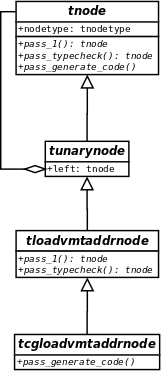
\includegraphics[width=150px]{./uml/cgnodeexample.png}
\caption{Диаграмма наследования для класса tcgloadvmtaddrnode}
\label{tcgloadvmtaddrnode}
\end{figure}

\pagebreak

\subsubsection{Таблицы символов}

Таблица символов это структура данных, которая используется компилятором для хранения 
информации о конструкциях исходной программы. Информация последовательно накапливается во время
разбора синтаксических конструкций. Далее она используется на этапе семантического анализа 
для проверки соответствия типов и при генерации кода для получения информации о расположении данных.

Записи в таблице символов содержат информацию об идентификаторах, такую как их
символьные строки, тип, область видимости, местоположение в памяти и прочую связанную
с ними информацию. FPC использует таблицы символов для хранения информации о модулях,
константах и переменных, подпрограммах, структуре составных типов данных.

Таблицы символов и синтаксическое дерево тесно связаны: синтаксическое дерево описывает действия с
данными. Описание структуры данных хранятся в таблице символов.

\subsubsection{Трансформации синтаксического дерева}

Во время компиляции FPC неоднократно трансформирует полученное на этапе синтаксического 
анализа синтаксическое дерево. Это необходимо для:
\begin{itemize}
    \item Упрощения логики отдельных узлов синтаксического дерева. К 
примеру, узлы преобразования типов упрощают логику узлов загрузки значения переменных,
арифметических операций и др. выражений.
    \item Проведения машинно-независымой оптимизации. К примеру удаление недостижимого
кода.
    \item Реализации новых концепций языка через старые. К примеру, реализация
case of string\cite{misha} или доступ к локальным переменным объемлющей функции в
случае компиляции в байт-код.
\end{itemize}      

Возможность реализации новых концепций языка через старые можно использовать и
для реализации замыканий. Заметим, что замыкание отличаются от 
обычный подпрограммы наличием свободных переменных. Преобразование
замыкания в процедуру, не содержащую свободных переменных называется преобразованием
замыканий\cite{moderncompiler}.

Преобразование замыканий давно используется в языках программирования, основанных на
лямбда-исчислении. Прямая реализация модели подстановки
лямбда-исчисления приводит к многократному вычислению одних и тех же выражений.
Преобразованием замыканий позволяет избежать бесполезных вычислений
и улучшения производительности таких программ \cite{lambdaclosure95}. 
Функция со свободными переменными
заменяются фуцией с дополнительными параметром - окружением. Свободные переменные
в теле исходной функции заменятся ссылками на окружение.  
Неизменяемость переменных в лямбда-исчислении позволяет реализовать сохранение
переменных в окружение разными способами:

\iffalse TODO: руководителю не понравились эти пироги. Рассказать про наш случай, плевать
на функциональные языки. \fi

\begin{description}
    \item[Общее окружение] Замыкания, имеющие общие свободные переменные,
используют общее окружение. Во время выполнения программы по мере активации функций
из вновь созданных окружений необходимо составлять связный список.
Преимущество такого подхода - быстрое создание окружения и экономия памяти. Недостатком
является увеличение времени доступа к переменным, т.к. время доступа к элементам связного
списка пропорционально длине списка.
    \item[Плоское окружение] Для каждого замыкания создаётся отдельная структура данных,
содержащая значения всех необходимых переменных. Плюс такого подхода - быстрый доступ
к переменным окружения. Минус - долгое создание замыкания и дополнительный расход памяти.
\end{description}

Описанный подход преобразования замыканий применим к императивным языками
программирования. Статически типизированный язык программирования Scala
использует преобразования замыканий\cite{scalaoverview}\cite{scalaclosure}. То что
Scala использует статическую типизацию и допускает изменение переменных делает
язык очень похожими на Free Pascal. Главное отличие - полностью автоматическое
управление динамической памяти компилятором, решающее проблему управления памятью
созданных окружений.

\subsubsection{Заключительная стадия}

В FPC нет промежуточного представления кода, который начальная стадия
передавала бы в заключительную стадию. Вместо генерации промежуточного представления
начальная стадия во время обхода синтаксического дерева последовательно вызывают методы
высокоуровневого генератора кода. Такой подход очень похож на использование
промежуточного представления, но избавляет от необходимости генерировать промежуточные
структуры данных.

\iffalse TODO: рассказать почему генератор высокоуровневый и зачем здесь диаграмма. \fi

\begin{figure}[htb]
\centering
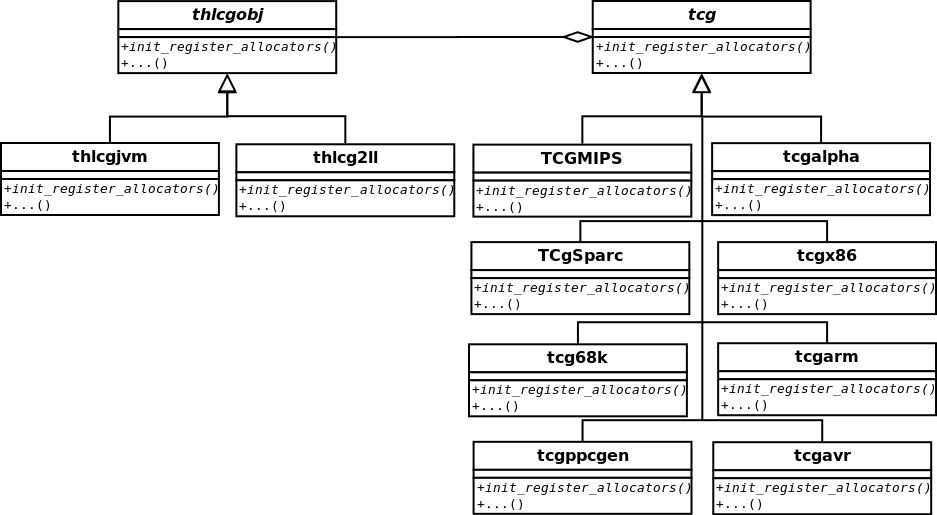
\includegraphics[width=\textwidth]{./uml/cgen.png}
\caption{Диаграмма классов генератора кода}
\end{figure}

\pagebreak

\section{Функциональные требования}

Компилятор должен:
\begin{enumerate}
    \item Позволять объявлять анонимные подпрограммы внутри тела других подпрограмм.
Синтаксис объявления анонимной подпрограммы такой же как и для обычной подпрограммы с двумя исключениями:
        \begin{itemize}
            \item после ключевых слов procedure и function нет имени подпрограммы, а сразу идет опциональный список формальных аргументов;
            \item после списка формальных аргументов (если он опущен, то после ключевых слов procedure или function) не ставится точка с запятой.
        \end{itemize}

         Пример 1:
\begin{lstlisting}
  procedure begin
    Writeln('inside');
  end;
\end{lstlisting}

         Пример 2:
\begin{lstlisting}
  procedure begin
    Writeln('inside');
  end;
\end{lstlisting}

    \item Позволять анонимным функциям возвращать значения, используя ключевое слово Result:

Пример:
\begin{lstlisting}
  function(num: Integer): Integer begin
    Result := num + 10;
  end;
\end{lstlisting}

    \item Запрещать анонимным процедурам использовать переменную Result объемлющей функции:

Пример:
\begin{lstlisting}
  function Calculate: Integer;
  begin
    ...
    procedure begin
      Result := 10; // Error, result can't be captured
    end;
  end;
\end{lstlisting}

    \item Позволять анонимным процедурам использовать переменные, объявленные в объемлющей функции:

Пример:
\begin{lstlisting}
  procedure Calculate: Integer;
  var num: Integer;
  begin
    ...
    procedure begin
      num := 10;
    end;
  end;
\end{lstlisting}

    \item Позволять анонимным процедурам использовать переменные, объявленные в объемлющей функции, при уровне вложенности больше 1:

Пример:
\begin{lstlisting}
  procedure Outer;
  var num: Integer;
    procedure Calculate;
    begin
      ...
      procedure begin
        num := 10;
      end;
    end;
  begin
   ...
\end{lstlisting}

    \item Продлевать время жизни захваченных переменных. Время жизни захваченной переменной определяется не временем работы функции, где она объявлена, а временем жизни всех ссылающихся на неё замыканий.

    \item Осуществлять захват переменных по ссылке. Замыкания, созданные в одном лексическом контексте должны иметь доступ к одним и тем же переменным.
      
    \item Корректно осуществлять проверку типов в момент присваивания значений переменным-указателям на замыкание.

    \item Корректно осуществлять проверку типов во время вызова замыкания.
      
\end{enumerate}


\section{Требования к интерфейсу}

Компилятор имеет интерфейс командной строки, который описан
в руководстве пользователя FPC\cite{userguide}. Интерфейс остаётся неизменным.

\iffalse TODO: описать сообщения об ошибках \fi

\section{Проект}

\subsection{Средства реализации}

\iffalse TODO: сомнительно \fi

Проект использует язык программирования Free Pascal. Редактирование исходных кодов
компилятора возможно с использованием любого текстового редактора. Тем не менее
для работы с проектом большого размера предпочтительно использование редактора с
поддержкой навигации по коду. Возможность быстрого перехода к объявлению и описанию
идентификаторов упрощает поиск нужной информации и ускоряет процесс разработки.
Было рассмотрено несколько кандидатов:
\begin{description}
  \item[Free Pascal's text mode IDE] Приемущества: находится в репозитории с 
компилятором. Недостатки: отсутствует графический интерфейс, отсутствует
быстрый переход к определению переменных.
  \item[Emacs] Приемущества: мощный текстовый редактор, поддерживающий большое
количество расширений. Недостатки: переход к определению переменных не работает
с исходными кодами FreePascal.
  \item[Lazarus] Преимущества: удобный графический пользовательский интерфейс.
Корректный быстрый переход к определению символов. Настраиваемые горячие клавиши.
В репозитории компилятора есть файл проекта для Lazarus.
  \item[MSEide] Преимущества: быстрый. Недостатки: неудобный 
пользовательский интерфейс.
\end{description} 
В итоге принято решение использовать среду разработки Lazarus, так как она
лучше всего подходит для работы с большим программным проектом на
языке программирования Free Pascal. Lazarus корректно разбирает
исходный код и предоставляет пользователю возможность удобной и
быстрой навигации по коду.

\subsection{Структуры данных}

Ключевые структуры данных: определения типов, таблицы символов и
синтаксическое дерево. Программа на языке программирования Free Pascal имеют рекурсивную структуру,
поэтому упомянутые структуры данных имеют сложные циклические зависимости. Пример такой 
зависимости: узел синтаксического дерева, представляющий обращение к перменной содержит имя
переменной. По имени переменной доступен её тип. Типом переменной может быть класс, который
содержит метод. Реализация метода  может содержать обращение к переменной.

Таблицы символов отдельно хранят определения типов и символьные имена. Существуют 
различные таблицы символов: таблица символов модуля, локальная таблица символов, таблица
символов, содержащая параметры процедуры и др. Все таблицы символов унаследованы от общего
базового класса TSymTable, определяющего для них общий интерфейс. Любая таблица символов отдельно
хранит определения типов и литеральные имена, что отражено на рис.~\ref{symboltable-sym-def}.
Таким образом, таблицы символов содержит доступные в текущем лексическом контексте
именованные объекты и соответствующие им типы.

\begin{figure}[htb]
\centering
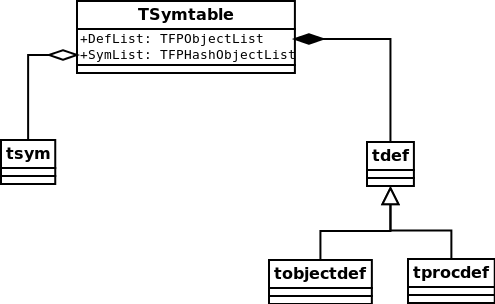
\includegraphics[width=300px]{./uml/sym-def-def-inheritence.png}
\caption{Диаграмма классов}
\label{symboltable-sym-def}
\end{figure}

На рис.~\ref{symboltable-sym-def} показаны 2 конкретных класса, унаследованных от
абстрактного класса tdef. Первый из них, tobjectdef, хранит информацию о классе: 
его родитель, реализованные интерфейсы, список методов, список полей и др. Второй, tprocdef, хранит
информацию о типе процедуры: список аргументов, тип возвращаемого значения, локальные
переменные. Отметим, что tprocdef и tobjectdef содержат
список именованных объектов, каждый из которых, тоже имеет тип. Это отражено на
рис.~\ref{symtable-def}, определения типов объекта и процедуры содержат таблицы символов. Причем,
они используют разные конкретные реализации.

\begin{figure}[htb]
\centering
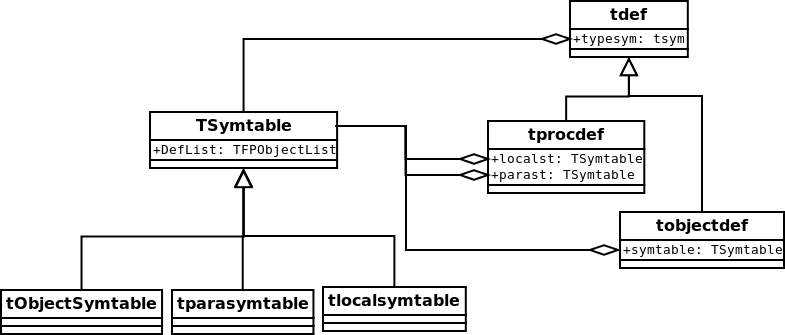
\includegraphics[width=\textwidth]{./uml/symtable-def.png}
\caption{Диаграмма классов}
\label{symtable-def}
\end{figure}

Литеральные имена, используемые для доступа к типам, называются символами. На
рис.~\ref{sym-def-sym-inheritence} изображена диаграмма классов для нескольких символов и 
их связь с определениями типов. Каждый символ унаследован от общего класса tsym. Конкретные
реализации рассчитаны для работы с конкретными определениями типов. К примеру, 
из-за того, что Free Pascal поддерживает перегрузку операторов, может существовать несколько
подпрограмм с одним именем и разными определениями. Поэтому tprocsym хранит список ссылок на 
определения типов подпрограмм. В это же время ttypesym содержит только одну ссылку на
определение типа.

\begin{figure}[htb]
\centering
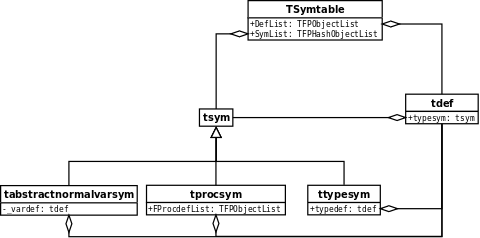
\includegraphics[width=\textwidth]{./uml/sym-def-sym-inheritence.png}
\caption{Диаграмма классов}
\label{sym-def-sym-inheritence}
\end{figure}

Теперь рассмотрим связь синтаксического дерева и таблицы символов. Если таблицы символов отражают
информацию о именованных данных, то синтаксическое дерево отражает информацию о действиях. 
Обращение к переменной является примером действия с именованными данными. Синтаксический
узел, отражающий обращение к переменной - tloadnode. На рис.~\ref{sym-node} показано, как tloadnode
хранит информацию о переменной.

\begin{figure}[htb]
\centering
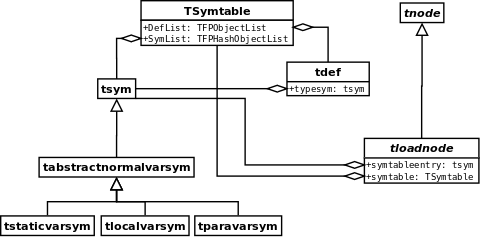
\includegraphics[width=\textwidth]{./uml/sym-node.png}
\caption{Диаграмма классов}
\label{sym-node}
\end{figure}

Кроме ссылок из узлов синтаксического дерева на именованные объекты теоретически возможна обратная
ситуация. Подпрограммы имеют реализацию, которую компилятор обрабатывает в виде синтаксического
дерева. К счастью определение типа подпрограммы не содержит ссылок на тело подпрограммы. Связь
реализации и информации о типе подпрограммы показана на рис.~\ref{tprocinfo}

\begin{figure}[htb]
\centering
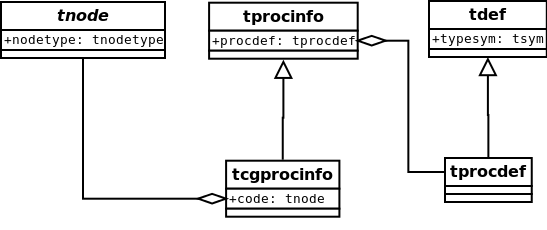
\includegraphics[width=400px]{./uml/tprocinfo.png}
\caption{Диаграмма классов}
\label{tprocinfo}
\end{figure}

\subsection{Модули и алгоритмы}

Самая большая сложность реализации замыканий заключается в управлению памятью. Захваченные переменные
не могут располагаться на стеке т.к. срок жизни переменных на стэке ограничен временем
работы объемлющей процедуры. Захваченные переменные необходимо располагать в куче. Память, однажды
выделенную под захваченные переменные позднее необходимо освобождать. С определением момента,
когда можно освобождать память замыкание есть несколько сложностей. Во-первых 
захват переменных по ссылке делает возможной ситуацию, когда несколько замыканий ссылаются 
на одни и те же переменные. Поэтому общие данные можно освобождать только когда все замыкания,
ссылающиеся на них становятся недоступными для вызова. Во-вторых, замыкания
могут быть объявлены в списке фактических аргументов другой функции. В случае ручного управления 
памятью пользователям языка программирования необходимо будет устанавливать договорённости
о том вызывающая или вызываемая сторона освобождает память. Это сделает использование замыканий
источником сложностей и ошибок.

Чтобы избежать ошибок, замыкание необходимо сделать управляемым типом данных, т.е.
типом данных с автоматическим управлением динамической памятью. К счастью, FPC уже содержит
сборщик мусора, использующий счётчик ссылок, который следит за объектами управляемых
типов данных. Управляемыми типами являются 
большинство реализаций строк, динамические массивы, COM-интерфейсы, Dispatch-интерфейсы, Variant и
составные типы данных, содержащие или унаследованные от управляемых типов данных.

Вместо того, чтобы реализовывать поддержку нового управляемого типа данных, для реализации
замыканий можно воспользоваться существующими COM-интерфейсами. Такой подход существенно
снижает сложность реализации, т.к. поддержка нового управляемого типа данных требует внесения
изменений в компилятор и библиотеку времени исполнения. Напротив, трансформация новых синтаксических
конструкций в существующие помогает уменьшить размер генератора кода. Это упрощает
поддержку нескольких целевых платформ, что особенно актуально для FPC. Реализация замыканий 
с использованием COM-интерфейсов не потребует изменений в генераторе кода и библиотеке
времени исполнения.

\subsubsection{Реализация замыканий с использованием COM-интерфейсов}

Рассмотрим реализацию замыканий с использованием COM-интерфейсов на примере:

\begin{lstlisting}
var p: reference to procedure;
begin
  i := procedure begin
          Writeln('inside');
       end;
  i();
end.
\end{lstlisting}

\paragraph{Объявление переменной}

Ключевая идея данного подхода в том, чтобы использовать COM-интерфейс в качестве переменной-указателя
на замыкание. Такой интерфейс содержит единственный метод Apply, имеющий сигнатуру, указанную
в объявлении переменной после ключевых слов "reference to". Назовём его интерфейс указателя на
замыкания.

\begin{lstlisting}
var p: reference to procedure;
\end{lstlisting}

\paragraph{Анонимная функция}

Для хранения захваченных переменных во время выполнения
создаётся специальный объект-хранилище. Время создания хранилища
и доступ к захваченным переменным обсуждается ниже. Пока что будем считать, что каждая анонимная
подпрограмма во время выполнения имеет связанный с ней объект-хранилище, через
который осуществляется доступ к локальным переменным.
Анонимная подпрограмма становится методом объекта-хранилища. Создаётся интерфейс, содержащий
единственную функцию Apply, имеющую такую же сигнатуру, как и анонимная функция. Объект-хранилище
реализует данный интерфейс, реализацией единственного метода Apply становится только что
разобранный анонимный метод.

Назовём только что описанный интерфейс интерфейсом реализации анонимного метода. Отметим, что
интерфейс реализации анонимного метода содержит единственный метод Apply. Вызов этого метода
приводит к вызову анонимной функции, в качестве скрытого параметра которой
передаётся объект-хранилище, содержащий захваченные переменные.

\begin{lstlisting}
       procedure begin
          Writeln('inside');
       end;
\end{lstlisting}


\paragraph{Присваивание}

Определение анонимной функции является выражением. Оно должно возвращать значение, которое
используется для вызова замыкания. Таким значением является интерфейс реализации анонимного
метода. Отметим, что интерфейсы реализации и указателя на анонимный метод имеют одинаковую
структуру. Оба интерфейса имеют единственный метод, имеющий одну и ту же сигнатуру. 
Это означает, что типы совместимы и возможно присваивание.

\begin{lstlisting}
  i := procedure begin
          Writeln('inside');
       end;
\end{lstlisting}

\paragraph{Вызов}

Для вызова замыкания необходимо вызвать единственный метод Apply интерфейса указателя на замыкание.

\begin{lstlisting}
  i();
\end{lstlisting}

\subsubsection{Сохранение захваченных переменных}

Хранилище создаётся для каждой функции, содержащей замыкания. Если необходимо
осуществлять доступ к переменным объемлющей функции, то, кроме захваченных
переменных текущей функции, оно содержит ссылку на хранилище объемлющей функции.

На примере ниже первое хранилище для локальных переменных будет создано в момент вызова процедуры
Outer. Оно будет содержать захваченную
переменную a. Второе хранилище будет создано в момент вызова процедуры Inner. Оно будет
хранить переменную b и ссылку на хранилище объемлющей функции.

\begin{lstlisting}
procedure Outer;
var a: Integer;
  procedure Inner;
  var p: reference to procedure;
      b: Integer;
  begin
    p := procedure begin
           Writeln(a + b);
         end;
  end;
begin
  Inner;
end;
  
\end{lstlisting}

\subsection{Стандарт кодирования}

Стандарт кодирования описан в документации проекта\cite{codingstyle}:
\begin{itemize}
  \item Ключевые слова пишутся маленькими буквами.
  \item Символы табуляции запрещены.
  \item Не следует отделять операторы, запятые и скобки пробелами.
  \item Размер отступов: 2 пробела для каждого уровня отступа.
  \item Перед блоком begin ... end следует делать отступы.
  \item Подпрограммы разделяют двумя пустыми строчками.
  \item У идущих подряд условных операторов следует писать else и последующее if 
на одной строке.
\end{itemize}

\section{Реализация и тестирование}

Предоставленный разработчикам патч содержит 1255 добавленных строк кода, 812 удалённых строк.
Так же добавлено 20 тестов общим объёмом 504 стоки. Изменения получили положительные отзывы
среди разработчиков\cite{mantis}.

\pagebreak

\section*{Заключение}
\addcontentsline{toc}{section}{Заключение}

Таким образом в процессе выполнения дипломной работы мною были углублены
знания о компиляторах современных языков программирования, улучшены навыки
поддержки и развития больших программных проектов. Я получил опыт участия в 
международном проекте с открытым исходным кодом и пообщался с опытными разработчиками.
Мною была рассмотрены различные общие подходы к реализации замыканий и разработано
решение для конкретного компилятора FPC.

Итогом работы стала пробная реализация, позволившая оценить сложность реализации 
замыканий, положительные и отрицательные черты выбранного подхода.
Созданная реализация должна
стать прототипом для окончательной понятной, стабильной и задокументированной
реализации замыканий для компилятора FPC.

\pagebreak

\begin{thebibliography}{99}
\bibitem{dragonbook} Альферд~В.~Ахо, Моника~С.~Лам, Рави~Сети, Джеффри~Д. Ульман. Компиляторы. Принципы, технологии и инструментарий. - 2 изд. - Вильямс, 2008. - 1184 с.
\bibitem{gof} Гамма~Э., Хелм~Р., Джонсон~Р., Влиссидес~Д. Приемы объектно-ориентированного проектирования. Паттерны проектирования, Спб.:Питер, 2010, 386 c.
\bibitem{misha} Денисенко М. В., Кленин А. С. Курсовая работа «Доработка компилятора Free Pascal: case of string». - ДВГУ, 2009г.
\bibitem{anonymmethods} Документация Delphi: Anonymous methods \url{http://docwiki.embarcadero.com/RADStudio/XE3/en/Anonymous_Methods_in_Delphi}
\bibitem{delhpimanged} Документация Delphi: System.Rtti.IsManaged \url{http://docwiki.embarcadero.com/Libraries/XE4/en/System.Rtti.IsManaged}
\bibitem{kaspersky} Крис Касперски, Техника оптимизации программ. Эффективное использование памяти. - БХВ-Петербург, 2003г. - 464с.
\bibitem{moderncompiler} Andrew~W.~Appel. Modern Compiler Implementation in Java. - 2nd edition - Cambridge University Press, 2004. - 512с.
\bibitem{fpc} Free Pascal Compiler \url{http://www.freepascal.org/}
\bibitem{codingstyle} Free Pascal Documentation. Coding style \url{http://wiki.freepascal.org/Coding_style}
\bibitem{fpctargets} Freepascal Wiki: Platform list \url{http://wiki.freepascal.org/Platform_list}
\bibitem{lazarus} Lazarus \url{http://www.lazarus.freepascal.org/}
\bibitem{scalaoverview} Martin Odersky and others. An Overview of the Scala Programming Language. - 2nd edition - Ecole Polytechnique Federale de Lausenne, 2001г. - 20c.
\bibitem{userguide} Michaël Van Canneyt, Florian Klämpfl. Free Pascal : User’s Guide. 2013 \url{http://www.freepascal.org/docs-html/user/user.html}
\bibitem{scalaclosure} Miguel Garcia. Code walkthrough of the UnCurry phase (Scala 2.8). Hamburg University of Technology, 2009г. - 5с.
\bibitem{engineeringcompiler} Keith~D.~Cooper, Linda Torczon. Engineering a Compiler. - 2nd edition - Morgan Kaufmann Publishers, 2012. - 801c.
\bibitem{cpp} Standard for Programming Language C++ \url{http://www.open-std.org/jtc1/sc22/wg21/docs/papers/2012/n3485.pdf}
\bibitem{lambdaclosure95} Yasuhiko~M., Greg~M., Robert~H. Typed  Closure Conversion. - Carnegie Mellon University, 1995. - 40c.

{\bf Обсуждения в системе контроля изменений fpc:}  
  
\bibitem{mantis} freepascal bugtracker. Issue\#0024481: Implement closures \url{http://bugs.freepascal.org/view.php?id=24481}
  
{\bf Обсуждения в списке рассылок разработчиков fpc (fpc-devel):}

\bibitem{sven1} Sven's comment - \url{http://lists.freepascal.org/lists/fpc-devel/2013-March/031595.html}
\bibitem{Marko1} Marko's comment - \url{http://lists.freepascal.org/lists/fpc-devel/2013-March/031657.html}


  
\end{thebibliography}
\addcontentsline{toc}{section}{Список литературы}

\pagebreak

\noindent Автор работы \superunder{\hrulefill}{\hspace{2cm}(подпись)\hspace{2cm}} (Ф.И.О.)\\

\noindent{}Квалификационная работа допущена к защите\\

\noindent{}Назначен рецензент\\
\superunder{\hrulefill}{(Фамилия, И.О. рецензента, ученая степень, ученое звание)\hspace{5cm}}\\

\vspace{2\baselineskip}
\noindent\begin{tabular}{p{0.5\textwidth} p{0.45\textwidth}}
\parbox{8cm}{Зав. кафедрой информатики,\\ математического и компьютерного\\ моделирования} &
\hfill А.~Ю.~Чеботарев\\
\end{tabular}
\vspace{2\baselineskip}
\begin{flushright}
Дата <<\rule{1cm}{0.5pt}>>\rule{3cm}{0.5pt}\quad 2013 г.
\end{flushright}

\end{document}

